\section{Bandit Approach Methods}\label{sec:bandit_methods}

\todo{clean up this section because I've been cutting and pasting out of it into
earilier in the document}

\subsection{Transfemoral Prosthesis Design and Control}
In this study, we use a transfemoral prosthesis and high-level neuromuscular
control that we first presented in \citet{thatte2016toward}. We briefly review
improvements to the hardware design and control strategy here.

Our prosthesis design (\cref{fig:prosthesis_bandit_opt}a) features series
elastic actuators at both joints (SEAs \citep{pratt1995series}) that enable
accurate torque control. These actuators consist of brushless motors (knee:
Robodrive ILM85-13HS, ankle: ILM70-10HS) coupled to Harmonic Drive gear sets
(CSG-25-50 and CSG-20-100, respectively).  The actuators deliver peak torques of
\unit[170]{N-m} at both joints and peak speeds of \unitfrac[1.93]{rev}{s} at the
knee and \unitfrac[1.17]{rev}{s} at the ankle. Absolute encoders (2x Renishaw
Resolute at the knee and one Renishaw Resolute and one Netzer DS-25 at the
ankle) located on both sides of fiberglass leaf springs (Gordon Composites)
measure spring deflection and thereby joint torque. We mount an IMU (YEI
Technology 3-Space Sensor) to the user's ipsilateral thigh to estimate the thigh
angle with respect to the vertical axis.  We detect stance/swing transitions via
hall effect sensors that measure the deflection in the prosthesis' composite
foot (Freedom Innovations Pacifica-LP).  The completed prototype weighs about
\unit[6]{kg} and is donned by able-bodied subjects via an L-shaped adaptor.

The control of the prosthesis distinguishes between a lower level and a
behavioral level. At the lower level, each actuator is controlled by a SEA
controller \citep{schepelmann2012development} that regulates desired joint
torque by commanding desired motor velocity. The behavioral level generates the
desired joint torques for the knee and ankle. We further subdivide the behavior
level into its stance and swing components.

\subsection{Optimization method}\label{sec:bandit_optimization}

To optimize the control parameters of this neuromuscular transfemoral prosthesis
control for specific users, we frame the task as a $K$-armed dueling bandits
problem \citep{yue2012k}. In this formalism, at each iteration $t \in [1,\ldots
T]$ of the optimization, an algorithm chooses two options, referred to as
bandits, out of the set of $K$ possibilities, so as to minimize the total
cumulated regret over the iterations. The cumulated regret is defined as
\begin{align}
    R(T) = \zeta^* T - \frac{1}{2} \sum_{t=1}^T \funcsb{E}{\zeta_{1t} + \zeta_{2t}}
\end{align}
where $\zeta^*$, $\zeta_{1t}$, and $\zeta_{2t}$, are the values of the optimal
bandit and first and second bandits chosen on iteration $t$ respectively. To
minimize $R(T)$, algorithms must effectively trade of exploration of all bandits
to gain confidence in their values and exploitation of the best bandit so as to
not incur regret.

In a dueling bandits problem, we do not observe numeric rewards directly.
Rather, we observe if an oracle prefers the first bandit to the second.  Because
we never directly observe numeric values, algorithms for this problem use
alternative notions of value. In this work, we utilize the Double Thompson
sampling method \citep{wu2016double}, which achieves state-of-the-art regret on
several datasets. This method defines a bandit's value as its Copeland Score:
the number of other options that a bandit defeats on average.

Key to employing this method for prosthesis optimization is offline generation
of parameter sets for which we are likely to obtain reasonable gaits for
different subjects. This task can be viewed as sampling from the set of
parameters that produce gait patterns consistent with human locomotion. In this
work, we explore generating this set of controllers using a recently published
gait data set that includes kinematics and kinetics for individual subjects
walking at three different speeds, \unitfrac[0.8, 1.2, and 1.6]{m}{s}
\citep{moore2015elaborate}.  For each subject in this dataset, we use the
Covariance Matrix Adaptation Strategy \citep{hansen2006cma} to find
neuromuscular model parameters $\Gamma$ that reproduce the subject's
body-weight-normalized knee and ankle joint torques $\tau_\tn{h} =
[\tau_\tn{h}^\tn{k},\tau_\tn{h}^\tn{a}]^T$ given the subject's hip, knee, and
ankle angle trajectories $\theta_\tn{h} =
[\theta_\tn{h}^\tn{h},\theta_\tn{h}^\tn{k},\theta_\tn{h}^\tn{a}]^T$.
Specifically, we solve
\begin{align}
    \Gamma &= \argmin_\Gamma \left(\tau_\tn{h} - \tau_\tn{nm} \right)^T
    \left(\tau_\tn{h} - \tau_\tn{nm} \right) + \alpha \xi_\tn{nm}^T \xi_\tn{nm}
\end{align}
where $(\tau_\tn{nm}, \xi_\tn{nm}) = \func{neuro}[\Gamma][]{\theta_\tn{h}}$ are
the torques and muscle activations generated by the neuromuscular model given
the human joint angle trajectories and model parameters. $\alpha = 0.01$ is a
small constant we use to help regularize the solutions.

\Cref{tab:params} shows the parameters we optimize during this process.  For
each parameter in the Speed-Independent category, we look for a single value to
use across all speeds. For parameters in the Speed-Dependent category we search
for three different values, one for each gait speed in the dataset
(\unitfrac[0.8, 1.2, and 1.6]{m}{s}). The parameters we choose to optimize
include the isometric force and feedback gains for each muscle, which are
closely related to the effective stiffness of the
joint~\citep{geyer2003positive}, muscle prestimulations, which are related to
the stride energy~\citep{geyer2003positive}, and the muscle reference angles, to
help deal with the kinematic variability between
subjects~\citep{geyer2010muscle}.

From the dataset provided by \citet{moore2015elaborate}, which contains samples
for twelve subjects, we were able to extract nine parameter sets. (One subject's
torque data is corrupted and two subjects' data resulted in an overly flexed
knee when used on the prosthesis.) \Cref{fig:nm_fit} shows an example of two
subjects' torque patterns shown in red. We see that there are significant
differences between the two subjects in terms of both timing and magnitude of
torque. In green, we see that after optimizing the neuromuscular model for each
subject, it is able to capture both gait patterns. 

We can quantify the quality of the model fit to the data by computing the root
mean squared (RMS) error between the model's predicted torques and the actual
torques. Over the nine parameter sets we achieve a median RMS knee torque error
of 35\% of the RMS human knee torque, and a median RMS ankle torque error of
15\% of the RMS human ankle torque. Much of the error in the knee torque
prediction occurs right after heel strike, where the model typically predicts
near-zero torque. In future work we plan to adapt the model to produce more knee
flexion torque at heel strike, which should significantly reduce the model
error.

To compensate for kinematic differences between the prosthesis and the training
data, before sending prosthesis joint angles to the neuromuscular control, we
add constant bias angles to the joint encoder readings so that at joint $j$,
\begin{align}
    \theta_\tn{model}^j = \theta_\tn{encoder}^j + \theta_0^j.
    \label{eq:bias_param}
\end{align}
We hand-tune these bias parameters for each bandit and subject to ensure the
bandits work as well as possible.
 
\begin{margintable}[-3in]    
    \centering
    \small
    \begin{tabular}{ll|l}
        \multicolumn{2}{c|}{Speed-Independent} & Speed- \\
                                         &     & Dependent \\
        \midrule
        $F_\tn{max}^\tn{ham}$            & ham $\phi_0^\tn{hip}$   & $^{F+}G_\tn{ham}^\tn{ham}$   \\
        $F_\tn{max}^\tn{vas}$            & ham $\phi_0^\tn{knee}$  & $^{F+}G_\tn{vas}^\tn{vas}$   \\
        $F_\tn{max}^\tn{bfsh}$           & vas $\phi_0$            & $^{F+}G_\tn{gas}^\tn{gas}$   \\
        $F_\tn{max}^\tn{gas}$            & bfsh $\phi_0$           & $^{F+}G_\tn{sol}^\tn{sol}$   \\
        $F_\tn{max}^\tn{sol}$            & gas $\phi_0^\tn{knee}$  & $^{F-}G_\tn{sol}^\tn{ta}$    \\
        $F_\tn{max}^\tn{ta}$             & gas $\phi_0^\tn{ankle}$ & $^{L+}G_\tn{bfsh}^\tn{bfsh}$ \\
        $^\tn{off}l_\tn{bfsh}^\tn{bfsh}$ & sol $\phi_0$            & $^{L-}G_\tn{bfsh}^\tn{vas}$  \\
        $^\tn{off}l_\tn{bfsh}^\tn{vas}$  & ta  $\phi_0$            & $^{L+}G_\tn{ta}^\tn{ta}$     \\
        $^\tn{off}l_\tn{ta}^\tn{ta}$     & $S_0^\tn{vas}$          & \\
                                         & $S_0^\tn{ham}$          & \\
    \end{tabular}
    \caption[Parameters optimized to generate parameter sets for dueling bandits
    optimization]{Optimized parameters, $\Gamma$. Speed-independent parameters
    use a single value for all speeds, while speed dependent parameters have
    distinct values for \unitfrac[0.8, 1.2, and 1.6]{m}{s} gaits. Consequently,
    in total we optimize 43 parameters. $F_\tn{max}$ refers to a muscle's maximum
    isometric force, $\phi_0$ is a parameter used for muscle moment arm
    calculations, and $S_0$ is a muscle's pre-stimulation.}\label{tab:params}
\end{margintable}

\begin{figure}
    \centering 
    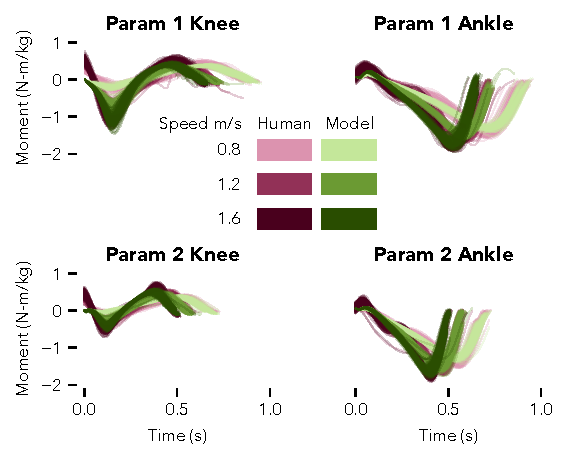
\includegraphics[width = \columnwidth]{nm_fit_w_legend.pdf}
    \caption{Results of the offline optimization that fits the neuromuscular
    model to intact-subject gait data. Shown are the knee and ankle torques for
    two different subjects. These plots show there can be significant
    inter-subject gait variability.}\label{fig:nm_fit}
\end{figure}

\subsection{Experiment Procedure}
In our experiment, we test the ability of our offline optimization approach to
generate controllers that are suited to different subjects and to produce
kinematics and kinetics similar to those of intact subjects. We further test the
effectiveness of using offline optimizations to help improve the ability of the
control to generalize to speeds different than those experienced during the
online optimization.

After providing informed consent to a protocol approved by the Carnegie Mellon
University Internal Review Board, five non-amputee subjects (four male, one
female, average mass = \unit[68.8]{kg} std \unit[11.17]{kg}) donned the
prosthesis via the able-bodied adaptor shown in
\cref{fig:prosthesis_bandit_opt}. On the contralateral leg, subjects wore a lift
shoe, the height of which we adjusted to ensure subjects' hips were even when
standing.

Subjects participated in a three day study. On the first day, subjects
acquainted themselves with the prosthesis for roughly 2 hours. By the end of
this period, all subjects were able to walk (while holding hand rails)
consistently without tripping on a set of hand-tuned parameters at a speed of up
to \unitfrac[1.2]{m}{s}. On the second day, the first 15 minutes consisted of
hand-tuning the bias angles for each parameter set (\cref{eq:bias_param}) to
allow the subject to achieve adequate ankle and knee flexion for as many
parameters as possible. Then, we performed the dueling bandits optimization for
50 iterations, which required approximately thirty minutes of walking at
\unit[0.8]{m/s}. Each iteration consisted of roughly ten seconds of walking on
each parameter, after which the subject indicated their preference. If subjects
were unsure of their decision they could walk with both parameter sets multiple
times. If their uncertainty persisted, the experimenter chose the parameter set
that produced angles and torques more aligned with human data.  If the
experimenter also had no preference, a random number generator selected the
winner. We chose to perform fifty iterations, as pilot testing suggested this
was sufficient for the algorithm to begin comparing the optimal parameter set to
itself, indicating a high level of confidence in the optimum.

On the third day, subjects walked with their preferred parameters at
\unitfrac[0.8, 1.0, 1.2, 1.4, and 1.6]{m}{s}. For each speed, we tested both the
appropriate speed-dependent parameters and those designed for
\unitfrac[0.8]{m}{s}. To obtain parameters for \unitfrac[1.0 and 1.4]{m}{s} we
performed linear interpolation between the adjacent parameters.  Finally, we
recorded the subject's gait at \unitfrac[0.8]{m}{s} for all non-preferred
parameter sets and the hand-tuned parameters used on the first day. 
